\documentclass[11pt]{article}
\usepackage[utf8]{inputenc}
\usepackage[dvips]{graphicx}
\usepackage{fancybox}
\usepackage{verbatim}
\usepackage{array}
\usepackage{latexsym}
\usepackage{alltt}
\usepackage{hyperref}
\usepackage{textcomp}
\usepackage{color}
\usepackage{amsmath}
\usepackage{amsfonts}
\usepackage{tikz}
\usepackage{float}
\usepackage[hmargin=3cm,vmargin=5.0cm]{geometry}
%\topmargin=0cm
\topmargin=-2cm
\addtolength{\textheight}{6.5cm}
\addtolength{\textwidth}{2.0cm}
%\setlength{\leftmargin}{-5cm}
\setlength{\oddsidemargin}{0.0cm}
\setlength{\evensidemargin}{0.0cm}


\begin{document}

\section*{Student Information } 
%Write your full name and id number between the colon and newline
%Put one empty space character after colon and before newline
Full Name : Furkan Göksel \\
Id Number : 2237436 \\

% Write your answers below the section tags
\section*{Answer 1}
\subsection*{a}     
\begin{figure}[H]
	\centering
	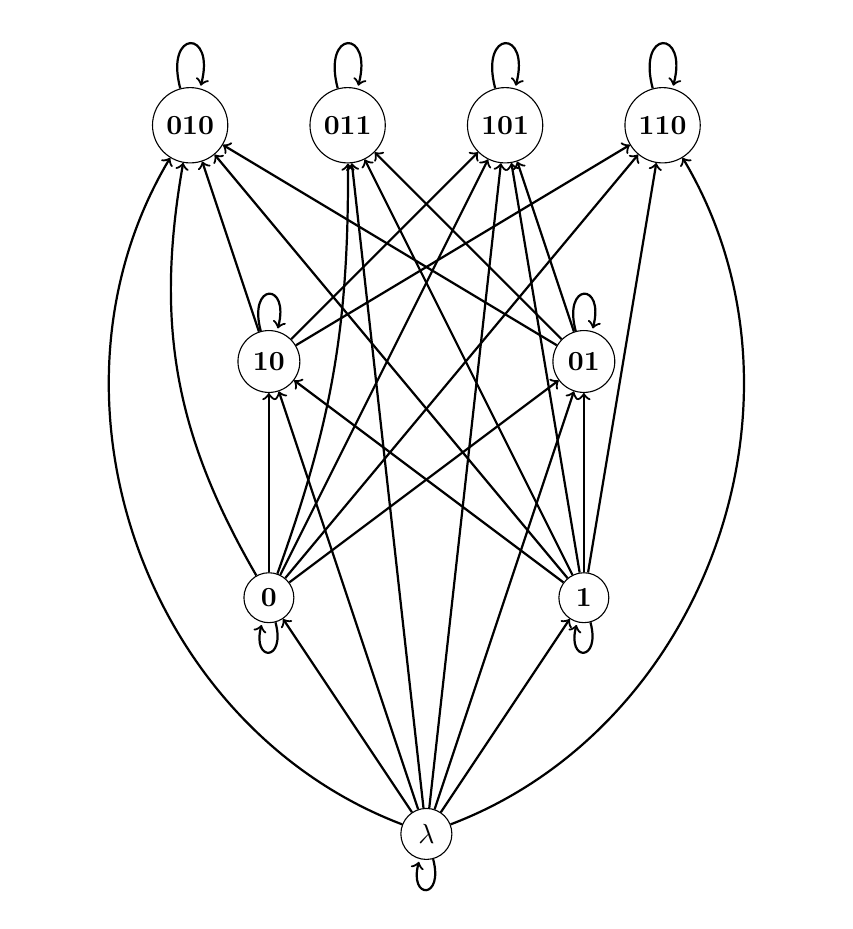
\begin{tikzpicture}
	
	\node[shape=circle,draw=black] (a) at (0,-3)     {\textbf{$\lambda$}};
	\node[shape=circle,draw=black] (b) at (-2,0)     {\textbf{0}};
	\node[shape=circle,draw=black] (c) at (2,0)     {\textbf{1}};
	\node[shape=circle,draw=black] (d) at (-2, 3)     {\textbf{10}};
	\node[shape=circle,draw=black] (e) at (2, 3)     {\textbf{01}};
	\node[shape=circle,draw=black] (f) at (-3, 6)     {\textbf{010}};
	\node[shape=circle,draw=black] (g) at (-1, 6)     {\textbf{011}};
	\node[shape=circle,draw=black] (h) at (1, 6)     {\textbf{101}};
	\node[shape=circle,draw=black] (i) at (3, 6)     {\textbf{110}};

	\path[->, thick] (a) edge [loop below] (a);
	\path[->, thick] (b) edge [loop below] (b);
	\path[->, thick] (c) edge [loop below] (c);
	\path[->, thick] (d) edge [loop above] (d);
	\path[->, thick] (e) edge [loop above] (e);
	\path[->, thick] (f) edge [loop above] (f);
	\path[->, thick] (g) edge [loop above] (g);
	\path[->, thick] (h) edge [loop above] (h);
	\path[->, thick] (i) edge [loop above] (i);
	\path[->, thick] (a) edge (b);
	\path[->, thick] (a) edge (c);
	\path[->, thick] (a) edge (d);
	\path[->, thick] (a) edge (e);
	\path[->, thick] (a) edge [bend left=50] (f);
	\path[->, thick] (a) edge (g);
	\path[->, thick] (a) edge (h);
	\path[->, thick] (a) edge [bend right=50] (i);
	\path[->, thick] (b) edge (d);
	\path[->, thick] (b) edge (e);
	\path[->, thick] (c) edge (d);
	\path[->, thick] (c) edge (e);
	\path[->, thick] (b) edge [bend left = 20] (f);
	\path[->, thick] (b) edge [bend right = 10] (g);
	\path[->, thick] (b) edge (h);
	\path[->, thick] (b) edge (i);
	\path[->, thick] (c) edge (f);
	\path[->, thick] (c) edge (g);
	\path[->, thick] (c) edge (h);
	\path[->, thick] (c) edge (i);
	\path[->, thick] (d) edge (f);
	\path[->, thick] (d) edge (h);
	\path[->, thick] (d) edge (i);
	\path[->, thick] (e) edge (f);
	\path[->, thick] (e) edge (g);
	\path[->, thick] (e) edge (h);
	
	\end{tikzpicture} 
\end{figure}
\subsection*{b}
S=$\{ \lambda,0,1,10,01,010,011,101,110 \}$ \\
In order to prove (S,R) is a poset, we have to show that R on the set S is reflexive, anti-symmetric and transitive. \\
1-\textbf{Reflexive}: R is reflective since (a,a) in R for every element in S. We can easily see that in the graph each element has a loop. \\
2-\textbf{Anti-symmetric}:For all pairs in relation, there is no such elements in R like (a,b,(b,a) and b$\neq$ a. It can be seen in graph. \\
3-\textbf{Transitive}: R is transitive since each pair in R such that for (a,b) and (b,c), there exist (a,c) in R for all pairs. This can be seen in graph.  
\subsection*{c}
The elements a and b of a poset (S, $<$) are called comparable if either a $<$ b or b $<$ a. When
a and b are elements of S such that neither a $<$ b nor b $<$ a, a and b are called incomparable, and 
when every two elements in the set are comparable, the relation is called a
total ordering. This relation is not total ordering because for example 010 and 101 are incomparable since 010 R 101 and 101 R 010 is false. 
\subsection*{d}

\begin{figure}[H]
	\centering
	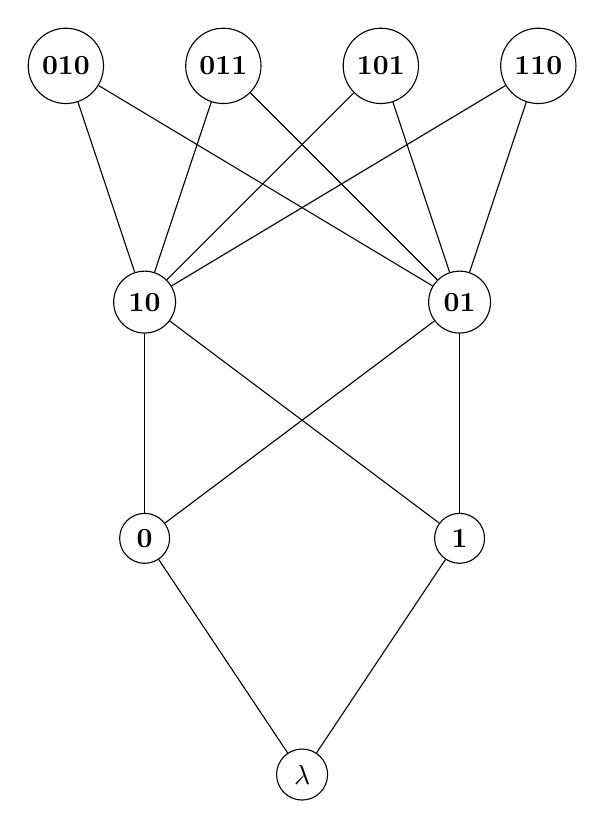
\begin{tikzpicture}[every loop/.style={}]
	
	\node[shape=circle,draw=black] (a) at (0,-3)     {\textbf{$\lambda$}};
	\node[shape=circle,draw=black] (b) at (-2,0)     {\textbf{0}};
	\node[shape=circle,draw=black] (c) at (2,0)     {\textbf{1}};
	\node[shape=circle,draw=black] (d) at (-2, 3)     {\textbf{10}};
	\node[shape=circle,draw=black] (e) at (2, 3)     {\textbf{01}};
	\node[shape=circle,draw=black] (f) at (-3, 6)     {\textbf{010}};
	\node[shape=circle,draw=black] (g) at (-1, 6)     {\textbf{011}};
	\node[shape=circle,draw=black] (h) at (1, 6)     {\textbf{101}};
	\node[shape=circle,draw=black] (i) at (3, 6)     {\textbf{110}};
	

	\path[-] (a) edge (b);
	\path[-] (a) edge (c);
	\path[-] (b) edge (d);
	\path[-] (b) edge (e);
	\path[-] (c) edge (d);
	\path[-] (c) edge (e);
	\path[-] (d) edge (f);
	\path[-] (d) edge (g);
	\path[-] (d) edge (h);
	\path[-] (d) edge (i);
	\path[-] (e) edge (f);
	\path[-] (e) edge (g);
	\path[-] (e) edge (h);
	\path[-] (e) edge (i);
	\end{tikzpicture} 
\end{figure}
The least element is $\lambda$ and maximal elements are 010,011,101,110
\subsection*{e}
(S,R) is not lattice since for example 0 and 1 don't have no least upper bound.
\section*{Answer 2}
\subsection*{a}
\begin{table}[H]
\small
\centering
\caption{ Adjacency List Presentation for G }
\label{table:example}
\begin{tabular}{|c|c|}	%% specify column number and vertical lines
\hline 							%% line draw
\textbf{Vertex} & \textbf{Terminal Vertices}  \\
\hline 
\hline 
a & a,b,d \\ \hline			%% separate columns by &
b & c,d  \\ \hline
c & b \\ \hline
d & c \\ \hline
e & b,f \\ \hline
f & b,e,f \\ \hline
g & c,f \\ 
\hline 

\end{tabular}
\end{table}
\subsection*{b}
Rows and columns goes from a to g (ie. first row a , second row b , .... seventh row g, same as columns). \\
\[
\begin{bmatrix}
    1 & 1 & 0 & 1 & 0 & 0 & 0 \\
    0 & 0 & 1 & 1 & 0 & 0 & 0 \\
    0 & 1 & 0 & 0 & 0 & 0 & 0 \\
    0 & 0 & 1 & 0 & 0 & 0 & 0 \\
    0 & 1 & 0 & 0 & 0 & 1 & 0 \\
    0 & 1 & 0 & 0 & 1 & 1 & 0 \\
    0 & 0 & 1 & 0 & 0 & 1 & 0 
    
\end{bmatrix}
\]
\subsection*{c}
For a in degree is 1 (a) and out degree is 3 (a,b,d) \\
For b in degree is 4 (a,c,e,f) and out degree is 2 (c,d) \\
For c in degree is 3 (b,d,g) and out degree is 1 (b) \\
For d in degree is 2 (b,a) and out degree is 1 (c) \\
For e in degree is 1 (f) and out degree is 2 (b,f) \\
For f in degree is 3 (e,f,g) and out degree is 3 (b,e,f) \\
For g in degree is 0 and out degree is 2 (c,f)
\subsection*{d}
1)g-f-e-b-c \\
2)g-f-e-b-d \\
3)f-e-b-d-c \\
4)e-f-b-d-c \\
5)g-f-b-d-c \\
6)f-f-e-b-c 
\subsection*{e}
\begin{itemize}
\item c b d c
\item b d c b
\item f e f f
\item f f e f
\item e f f e
\item d c b d
\end{itemize}
\subsection*{f}
From the definition , in a directed graph if there is a path between every two vertices in the underlying undirected graph, which is the undirected graph obtained by ignoring the directions of the edges of the directed graph. In G, when we ignore the directions, we can easily say that every vertex is reachable by a path, therefore G is a weakly connected graph.
\subsection*{g}
From the definition, A strongly connected component (SCC) of a directed graph is a maximal strongly connected subgraph. If we split G maximal strongly subgraphs we can find strongly connected components
\begin{itemize}
\item The subgraph with vertices e and f and edges {e.f},{f,e}
\item The subgraph with vertices b, c and d and edges {b,d},{d,c},{c,b} and {b,c}
\item Vertex a with no edges
\item Vertex g with no edges
\end{itemize}
\subsection*{h}
By the theorem, path between two vertices and length k is the just (i,j)th entry of adjacent matrix $A^k$. So, adjacent matrix of H is 
\[
\begin{bmatrix}
    1 & 1 & 0 & 1  \\
    0 & 0 & 1 & 1  \\
    0 & 1 & 0 & 0  \\
    0 & 0 & 1 & 0  \\
    
\end{bmatrix}
\]
And $A^3$ is
\[
\begin{bmatrix}
    1 & 3 & 3 & 2  \\
    0 & 1 & 1 & 1  \\
    0 & 1 & 1 & 0  \\
    0 & 0 & 1 & 1  \\
    
\end{bmatrix}
\] 
So if we sum the all entries we can find every distinct vertices path with length of 3. 1+3+3+2+1+1+1+1+1+1+1 = 16.
\section*{Answer 3}
\subsection*{a}
deg(a) = 2, deg(b)=6, deg(c)=4, deg(d) = 4, deg(e) = 6, deg(f) = 6, deg(g) = 4, deg(h) = 4, deg(i) =4, deg(j) = 6, deg(k) = 2\\
By the theorem, a connected multigraph has an Euler path if and only if it has exactly
two vertices of odd degree. (Theorem 2, page 697 of the textbook). Since there is no two vertices with odd degree, it doesn't have an Euler path.
\subsection*{b}
A graph has an Euler circuit if and only if the degree of every vertex is even. Since all vertices in the G have even degrees, we can easily say that G has a Euler Circuit.(Theorem 1, page 696 of the textbook). 
\subsection*{c}
We can easily see that one of the Hamiltonian path is a-b-e-h-i-f-c-j-k-g-d. Therefore G has a Hamiltonian path.
\subsection*{d}
if a vertex in the graph has degree two, then both edges that are incident with this vertex must be part of any Hamilton circuit, and note that when a Hamilton circuit is being constructed and this circuit has passed through a vertex, then all remaining edges incident with this vertex, other than the two used in the circuit, can be removed from consideration. From this, a's both two edges must be used, h's loop cannot be used then their right and top edge must be used, then e's top and bottom edge's will be used other edges can be removed, with this way for f, i and c vertices cannot be chosen edges with this method, since for each chosen path, either of these will be travelled twice which is not appropriate for Hamiltonian circuit. Hence G doesn't have a Hamiltonian circuit.
\section*{Answer 4}
\subsection*{a}
A complete bipartite graph $K_{m,n}$ is a graph that has its vertex set partitioned into two subsets of m and n vertices, respectively with an edge between two vertices if and only if one vertex is in the first subset and the other vertex is in the second subset. Total vertex number is m+n, and edges are since every vertex in subset 1 has an edge to every vertex in subset 2, and therefore each vertex in subset 1 has n edges and total m vertex in subset 1, so total edges is m*n.
\subsection*{b}
By inspection, $K_{m,n}$ with odd m and even n, when n > m, and starts with n's subset which is all vertices not connected to each other and when we traverse all vertices we will again in the n's subset and since there is no edges between vertices in these subset there is no Hamiltonian circuit, then starts with m's subset which is again all vertices not connected to each other, since this time to reach the last element we can't visit the all vertices in the n's subset and since same situation happens for m > n, it doesn't have Hamiltonian circuit.
\section*{Answer 5}
\subsection*{a}
\textbf{Initially} \\
S= $\{ \}$ \\
L(s) = 0 \\
L(u) = $\infty$\\
L(w) = $\infty$\\
L(v) = $\infty$\\
L(y) = $\infty$\\
L(x) = $\infty$\\
L(z) = $\infty$\\
L(t) = $\infty$\\ \\
\textbf{First Iteration} \\
S= $\{s \}$ \\
L(s) = 0 \\
L(u) = L(s) + W(s,u) = 4\\
L(w) = L(s) + W(s,w) = 3\\
L(v) = L(s) + W(s,v) = 5 \\
L(y) = $\infty$\\
L(x) = $\infty$\\
L(z) = $\infty$\\
L(t) = $\infty$\\ \\
\textbf{Second Iteration}\\
S= $\{ s,w \}$ \\
L(s) = 0 \\
L(u) = 4\\
L(w) = 3\\
L(v) = 5\\
L(y) = $\infty$\\
L(x) = L(w)+W(w,x) = 11\\
L(z) = L(w)+W(w,z) = 15\\
L(t) = $\infty$\\ \\
\textbf{Third Iteration}\\
S= $\{ s,w,u \}$ \\
L(s) = 0 \\
L(u) = 4\\
L(w) = 3\\
L(v) = 5\\
L(y) = L(u)+W(u,y) = 15\\
L(x) = 11\\
L(z) = 15\\
L(t) = $\infty$\\ \\
\textbf{Fourth Iteration}\\
S= $\{s,w,u,v \}$ \\
L(s) = 0 \\
L(u) = 4\\
L(w) = 3\\
L(v) = 5\\
L(y) = L(v)+W(v,y) = 11\\
L(x) = L(v)+W(v,x) = 6\\
L(z) = 15\\
L(t) = $\infty$\\ \\
\textbf{Fifth Iteration} \\
S= $\{s,w,u,v,x \}$ \\
L(s) = 0 \\
L(u) = 4\\
L(w) = 3\\
L(v) = 5\\
L(y) = L(x) + W(x,y) = 8\\
L(x) = 6\\
L(z) = L(x) + W(x,z) = 13\\
L(t) = $\infty$\\ \\
\textbf{Sixth Iteration} \\
S= $\{ s,w,u,v,x,y \}$ \\
L(s) = 0 \\
L(u) = 4\\
L(w) = 3\\
L(v) = 5\\
L(y) = 7\\
L(x) = 6\\
L(z) = L(y) + W(y,z) = 12\\
L(t) = L(y) + W(y,t) = 16\\ \\
\textbf{Seventh Iteration} \\
S= $\{ s,w,u,v,x,y,z \}$ \\
L(s) = 0 \\
L(u) = 4\\
L(w) = 3\\
L(v) = 5\\
L(y) = 7\\
L(x) = 6\\
L(z) = 12\\
L(t) = L(z) + W(z,t) = 15\\ \\
Therefore, after applying Dijkstra's algorithm shortest path from s to t has length is 15 and path is s-v-x-y-z-t.
\subsection*{b}
We should stop when we find n-1 edges which is 7 for this case.
\begin{table}[H]
\small
\centering
\begin{tabular}{|c|c|c|}	%% specify column number and vertical lines
\hline %% line draw
\textbf{Choice} & \textbf{Edge} & \textbf{Weight}  \\
\hline 
1 & $\{ x,y \}$ & 1 \\			%% separate columns by &
2 & $\{ x,v \}$ & 2 \\ 
3 & $\{ v,w \}$ & 3\\ 
4 & $\{ w,u \}$ & 1\\ 
5 & $\{ w,s \}$ & 3\\ 
6 & $\{ y,z \}$ & 4\\ 
7 & $\{ z,t \}$ & 3\\ 
\hline 
\end{tabular}
\end{table}
Total weight is 17.
\subsection*{c}
\textbf{Initial Case Minimum Spanning Tree} \\
\begin{figure}[H]
	\centering
	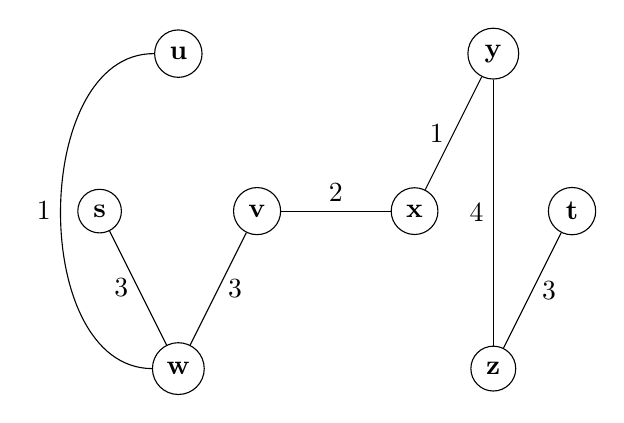
\begin{tikzpicture}
	\node[shape=circle,draw=black] (s) at (1, 2)     {\textbf{s}};
	\node[shape=circle,draw=black] (u) at (2, 4)     {\textbf{u}};
	\node[shape=circle,draw=black] (v) at (3, 2)     {\textbf{v}};
	\node[shape=circle,draw=black] (w) at (2, 0)     {\textbf{w}};
	\node[shape=circle,draw=black] (x) at (5, 2)     {\textbf{x}};
	\node[shape=circle,draw=black] (y) at (6, 4)     {\textbf{y}};
	\node[shape=circle,draw=black] (z) at (6, 0)     {\textbf{z}};
	\node[shape=circle,draw=black] (t) at (7, 2)     {\textbf{t}};

	\path[-] (u) edge [bend right=90] node[left]{1} (w); 
	\path[-] (v) edge node[above]{2} (x); 
	\path[-] (v) edge node[right]{3} (w); 
	\path[-] (w) edge node[left]{3} (s); 
	\path[-] (x) edge node[left]{1} (y); 
	\path[-] (y) edge node[left]{4} (z); 
	\path[-] (z) edge node[right]{3} (t); 
		
	\end{tikzpicture} 
\end{figure}
New edge (s,x,1) will be added to minimum span tree since it's weight is one of the smallest edge, however in order to add them we should delete v,w or s,w since if we don't delete this will be not tree because x-v-w-s-x is a simple circuit, and trees don't have simple circuits. \\
\textbf{After (s,x,1)} \\
\begin{figure}[H]
	\centering
	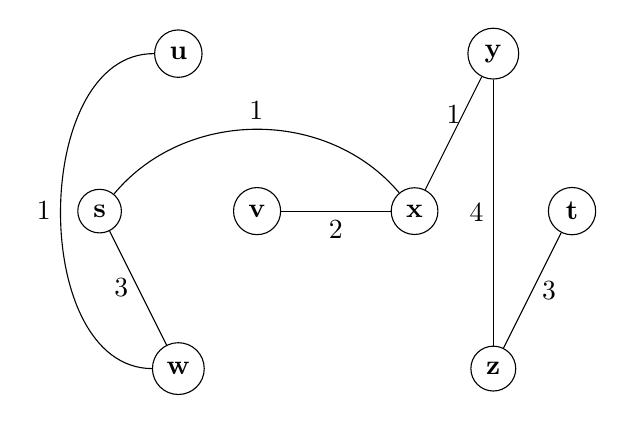
\begin{tikzpicture}
	\node[shape=circle,draw=black] (s) at (1, 2)     {\textbf{s}};
	\node[shape=circle,draw=black] (u) at (2, 4)     {\textbf{u}};
	\node[shape=circle,draw=black] (v) at (3, 2)     {\textbf{v}};
	\node[shape=circle,draw=black] (w) at (2, 0)     {\textbf{w}};
	\node[shape=circle,draw=black] (x) at (5, 2)     {\textbf{x}};
	\node[shape=circle,draw=black] (y) at (6, 4)     {\textbf{y}};
	\node[shape=circle,draw=black] (z) at (6, 0)     {\textbf{z}};
	\node[shape=circle,draw=black] (t) at (7, 2)     {\textbf{t}};

	\path[-] (u) edge [bend right=90] node[left]{1} (w); 
	\path[-] (v) edge node[below]{2} (x); 
	\path[-] (x) edge [bend right=50] node[above]{1} (s); 
	\path[-] (w) edge node[left]{3} (s); 
	\path[-] (x) edge node[above]{1} (y); 
	\path[-] (y) edge node[left]{4} (z); 
	\path[-] (z) edge node[right]{3} (t); 
		
	\end{tikzpicture} 
\end{figure}
Since it is the same after adding edge (t,u,6), we don't change the MST. \\
\textbf{After (t,u,6)} \\
\begin{figure}[H]
	\centering
	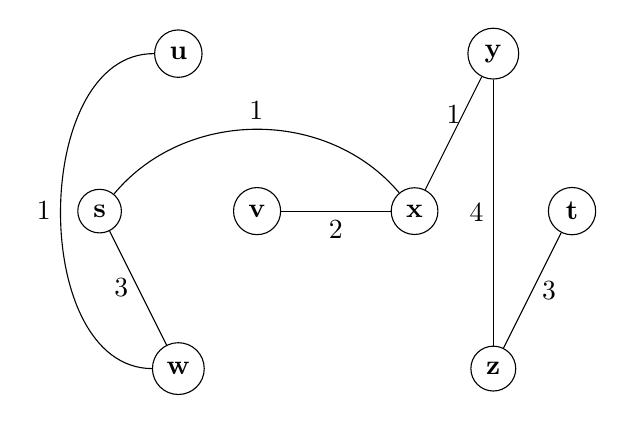
\begin{tikzpicture}
	\node[shape=circle,draw=black] (s) at (1, 2)     {\textbf{s}};
	\node[shape=circle,draw=black] (u) at (2, 4)     {\textbf{u}};
	\node[shape=circle,draw=black] (v) at (3, 2)     {\textbf{v}};
	\node[shape=circle,draw=black] (w) at (2, 0)     {\textbf{w}};
	\node[shape=circle,draw=black] (x) at (5, 2)     {\textbf{x}};
	\node[shape=circle,draw=black] (y) at (6, 4)     {\textbf{y}};
	\node[shape=circle,draw=black] (z) at (6, 0)     {\textbf{z}};
	\node[shape=circle,draw=black] (t) at (7, 2)     {\textbf{t}};

	\path[-] (u) edge [bend right=90] node[left]{1} (w); 
	\path[-] (v) edge node[below]{2} (x); 
	\path[-] (x) edge [bend right=50] node[above]{1} (s); 
	\path[-] (w) edge node[left]{3} (s); 
	\path[-] (x) edge node[above]{1} (y); 
	\path[-] (y) edge node[left]{4} (z); 
	\path[-] (z) edge node[right]{3} (t); 
		
	\end{tikzpicture} 
\end{figure}
We should add (s,z,-3) since it is one of the smallest edges, hence to preserve the tree property, we delete (y,z) edge. \\
\textbf{After (s,z,-3)} \\
\begin{figure}[H]
	\centering
	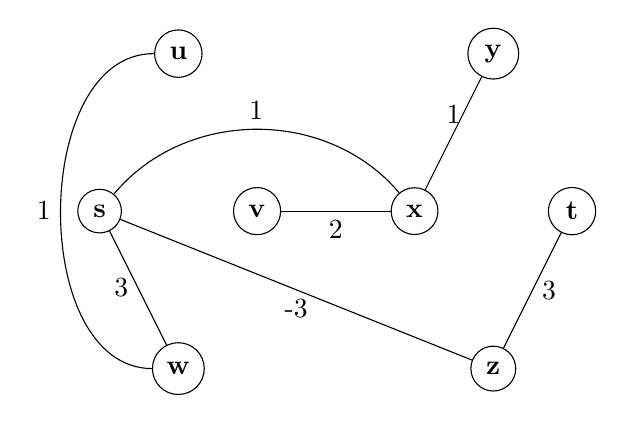
\begin{tikzpicture}
	\node[shape=circle,draw=black] (s) at (1, 2)     {\textbf{s}};
	\node[shape=circle,draw=black] (u) at (2, 4)     {\textbf{u}};
	\node[shape=circle,draw=black] (v) at (3, 2)     {\textbf{v}};
	\node[shape=circle,draw=black] (w) at (2, 0)     {\textbf{w}};
	\node[shape=circle,draw=black] (x) at (5, 2)     {\textbf{x}};
	\node[shape=circle,draw=black] (y) at (6, 4)     {\textbf{y}};
	\node[shape=circle,draw=black] (z) at (6, 0)     {\textbf{z}};
	\node[shape=circle,draw=black] (t) at (7, 2)     {\textbf{t}};

	\path[-] (u) edge [bend right=90] node[left]{1} (w); 
	\path[-] (v) edge node[below]{2} (x); 
	\path[-] (x) edge [bend right=50] node[above]{1} (s); 
	\path[-] (w) edge node[left]{3} (s); 
	\path[-] (x) edge node[above]{1} (y); 
	\path[-] (s) edge node[below]{-3} (z); 
	\path[-] (z) edge node[right]{3} (t); 
		
	\end{tikzpicture} 
\end{figure}
We don't have to add (u,y,3) since to add we should delete one of the edges from MST, we can delete s,w but not x,y since x,y is smaller than u,y. I don't add it to MST and shape will be preserved.\\
\textbf{After (u,y,3)} \\
\begin{figure}[H]
	\centering
	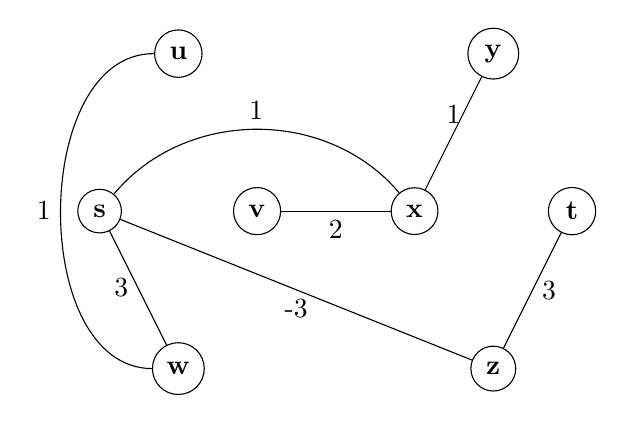
\begin{tikzpicture}
	\node[shape=circle,draw=black] (s) at (1, 2)     {\textbf{s}};
	\node[shape=circle,draw=black] (u) at (2, 4)     {\textbf{u}};
	\node[shape=circle,draw=black] (v) at (3, 2)     {\textbf{v}};
	\node[shape=circle,draw=black] (w) at (2, 0)     {\textbf{w}};
	\node[shape=circle,draw=black] (x) at (5, 2)     {\textbf{x}};
	\node[shape=circle,draw=black] (y) at (6, 4)     {\textbf{y}};
	\node[shape=circle,draw=black] (z) at (6, 0)     {\textbf{z}};
	\node[shape=circle,draw=black] (t) at (7, 2)     {\textbf{t}};

	\path[-] (u) edge [bend right=90] node[left]{1} (w); 
	\path[-] (v) edge node[below]{2} (x); 
	\path[-] (x) edge [bend right=50] node[above]{1} (s); 
	\path[-] (w) edge node[left]{3} (s); 
	\path[-] (x) edge node[above]{1} (y); 
	\path[-] (s) edge node[below]{-3} (z); 
	\path[-] (z) edge node[right]{3} (t); 
		
	\end{tikzpicture} 
\end{figure}
Since (w,z,-1) is one of the smallest edges, we should add it and in order to avoid simple path we should delete (s,w). \\
\textbf{After (w,z,-1)} \\
\begin{figure}[H]
	\centering
	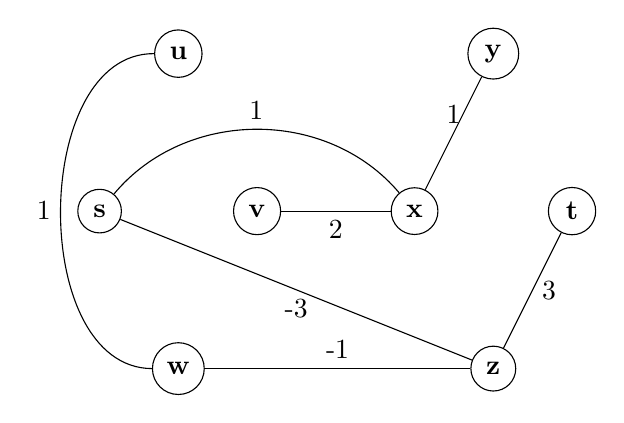
\begin{tikzpicture}
	\node[shape=circle,draw=black] (s) at (1, 2)     {\textbf{s}};
	\node[shape=circle,draw=black] (u) at (2, 4)     {\textbf{u}};
	\node[shape=circle,draw=black] (v) at (3, 2)     {\textbf{v}};
	\node[shape=circle,draw=black] (w) at (2, 0)     {\textbf{w}};
	\node[shape=circle,draw=black] (x) at (5, 2)     {\textbf{x}};
	\node[shape=circle,draw=black] (y) at (6, 4)     {\textbf{y}};
	\node[shape=circle,draw=black] (z) at (6, 0)     {\textbf{z}};
	\node[shape=circle,draw=black] (t) at (7, 2)     {\textbf{t}};

	\path[-] (u) edge [bend right=90] node[left]{1} (w); 
	\path[-] (v) edge node[below]{2} (x); 
	\path[-] (x) edge [bend right=50] node[above]{1} (s); 
	\path[-] (w) edge node[above]{-1} (z); 
	\path[-] (x) edge node[above]{1} (y); 
	\path[-] (s) edge node[below]{-3} (z); 
	\path[-] (z) edge node[right]{3} (t); 
		
	\end{tikzpicture} 
\end{figure}
\subsection*{d}
I think it can be done, if we consider new adding edge will be used and assume that this edge is (u,v) and we are trying to find shortest path from x to y, we can say that if we find x to u distance and v to y distance and we sum both and edge (u,v) it is possible to decide whether this path is short or not ($d((x,u))+c((u,v))+d((v,y))<d((x,y))$). Since at the beginning we applied Dijkstra's algorithm, we don't need to calculate again old edges' costs.
\section*{Answer 6}
\subsection*{a}
13 Vertices,12 Edges, and height is 4 since the largest path to leaf node is p to n which is 4 edges.
\subsection*{b}
w-s-m-t-q-x-n-y-u-z-v-r-p
\subsection*{c}
s-w-q-m-t-p-x-u-n-y-r-v-z
\subsection*{d}
p-q-s-w-t-m-r-u-x-y-n-v-z
\subsection*{e}
A Binary Tree is full if every node has 0 or 2 children. Since s has 1 child it is not a binary full binary tree.
\subsection*{f}
In binary search tree, the left subtree of a node contains only nodes with keys lesser than the node’s key, and 
the right subtree of a node contains only nodes with keys greater than the node’s key. Since $u > n$ and n is in the right subtree of u, T is not an binary search tree.
\subsection*{g}
Since empty tree's height is -1 and 1 node is 0, 4 node is necessary to construct full tenary tree (1 for root 3 for childs, left, mid ,right), then with this way h will be 1. For h=2 it is 7(1 root, 5 leaf node, 1 branch node), then when h is incremented by 1, it's number of nodes is incremented by 3. Therefore answer is 3h+1.
\subsection*{h}
\begin{figure}[H]
	\centering
	\begin{tikzpicture}
	
	\node[shape=circle,draw=black] (p) at (7, 7.5)     {\textbf{9}};
	\node[shape=circle,draw=black] (q) at (3, 5)     {\textbf{3}};
	\node[shape=circle,draw=black] (r) at (11, 5)     {\textbf{11}};
	\node[shape=circle,draw=black] (s) at (1, 2.5)     {\textbf{1}};
	\node[shape=circle,draw=black] (t) at (5, 2.5)     {\textbf{4}};
	\node[shape=circle,draw=black] (u) at (9, 2.5)    {\textbf{9}};
	\node[shape=circle,draw=black] (v) at (13, 2.5)     {\textbf{21}};
	\node[shape=circle,draw=black] (y) at (12, 0)     {\textbf{15}};
	\node[shape=circle,draw=black] (z) at (14, 0)     {\textbf{22}};
		
	\path[-] (p) edge (q);
	\path[-] (p) edge (r);
	\path[-] (q) edge (t);
	\path[-] (q) edge (s);
	\path[-] (r) edge (u);
	\path[-] (r) edge (v);
	\path[-] (v) edge (z);
	\path[-] (v) edge (y);
	\end{tikzpicture} 
\end{figure}
\subsection*{i}
\textbf{For 2}\\
$2<9$ : Go left subtree, $2<3$ : Go right subtree, $2>1$: Go right subtree, seeing empty then 2 is not in this tree. \\
\textbf{For 22}\\
$9<22$ : Go right subtree, $11<22$ : Go right subtree, $21 < 22$: Go right subtree, found.
\subsection*{j}
\begin{figure}[H]
	\centering
	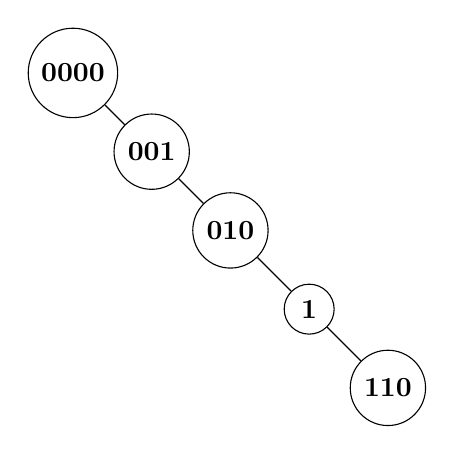
\begin{tikzpicture}
	
	\node[shape=circle,draw=black] (p) at (7, 7)     {\textbf{0000}};
	\node[shape=circle,draw=black] (q) at (8, 6)     {\textbf{001}};
	\node[shape=circle,draw=black] (r) at (9, 5)     {\textbf{010}};
	\node[shape=circle,draw=black] (s) at (10, 4)     {\textbf{1}};
	\node[shape=circle,draw=black] (t) at (11, 3)     {\textbf{110}};
		
	\path[-] (p) edge (q);
	\path[-] (q) edge (r);
	\path[-] (r) edge (s);
	\path[-] (s) edge (t);
	\end{tikzpicture} 
\end{figure}
\subsection*{k}
\textbf{For 001} \\
001 is alphabetically after the 000 so go right subtree, then we find 001. \\
\textbf{For 011} \\
011 is alphabetically after the 000 so go right subtree, 011 is alphabetically after the 001 so go right subtree, 011 is alphabetically after the 010 so go right subtree, 011 is alphabetically before the 1 so go left subtree, since it is empty 011 is not in this tree.
\subsection*{l}
\begin{figure}[H]
	\centering
	\begin{tikzpicture}
	
	\node[shape=circle,draw=black] (g) at (-2, 8)     {\textbf{g}};
	\node[shape=circle,draw=black] (f) at (-4, 6)     {\textbf{f}};
	\node[shape=circle,draw=black] (e) at (-6, 4)     {\textbf{e}};
	\node[shape=circle,draw=black] (b) at (-3, 4)     {\textbf{b}};
	\node[shape=circle,draw=black] (d) at (-3, 2)     {\textbf{d}};
	\node[shape=circle,draw=black] (c) at (-1, 6)     {\textbf{c}};	
	\node[shape=circle,draw=black] (a) at (2, 8)     {\textbf{a}};	
	\path[-] (g) edge (f);
	\path[-] (g) edge (c);
	\path[-] (f) edge (e);
	\path[-] (f) edge (b);
	\path[-] (b) edge (d);
	\end{tikzpicture} 
\end{figure}
\end{document}